%%%%%%%%%%%%%%%%%%%%%%% file template.tex %%%%%%%%%%%%%%%%%%%%%%%%%
%
% This is a general template file for the LaTeX package SVJour3
% for Springer journals.          Springer Heidelberg 2010/09/16
%
% Copy it to a new file with a new name and use it as the basis
% for your article. Delete % signs as needed.
%
% This template includes a few options for different layouts and
% content for various journals. Please consult a previous issue of
% your journal as needed.
%
%%%%%%%%%%%%%%%%%%%%%%%%%%%%%%%%%%%%%%%%%%%%%%%%%%%%%%%%%%%%%%%%%%%
%
% First comes an example EPS file -- just ignore it and
% proceed on the \documentclass line
% your LaTeX will extract the file if required
\begin{filecontents*}{example.eps}





%!PS-Adobe-3.0 EPSF-3.0
%%BoundingBox: 19 19 221 221
%%CreationDate: Mon Sep 29 1997
%%Creator: programmed by hand (JK)
%%EndComments
gsave
newpath
  20 20 moveto
  20 220 lineto
  220 220 lineto
  220 20 lineto
closepath
2 setlinewidth
gsave
  .4 setgray fill
grestore
stroke
grestore
\end{filecontents*}
%
\RequirePackage{fix-cm}
%
%\documentclass{svjour3}                     % onecolumn (standard format)
%\documentclass[smallcondensed]{svjour3}     % onecolumn (ditto)
%\documentclass[smallextended]{svjour3}       % onecolumn (second format)
\documentclass[twocolumn]{svjour3}          % twocolumn
%
\smartqed  % flush right qed marks, e.g. at end of proof
%
\usepackage{graphicx}
\usepackage{color}
\usepackage{listings}
\usepackage{fancyvrb}
\usepackage{url}
\usepackage{fix2col}
%\usepackage{natbib}
\usepackage{epsfig}
\usepackage{algorithm}
\usepackage{algorithmic}
%\input{highlight.sty}

\lstset{
basicstyle=\ttfamily \scriptsize,
language=java,
frame=single,
stringstyle=\ttfamily,
showstringspaces=false
}

\hyphenation{sche-me}
%
% \usepackage{mathptmx}      % use Times fonts if available on your TeX system
%
% insert here the call for the packages your document requires
%\usepackage{latexsym}
% etc.
%
% please place your own definitions here and don't use \def but
% \newcommand{}{}
%
% Insert the name of "your journal" with
% \journalname{myjournal}
%
\providecommand{\e}[1]{\ensuremath{\times 10^{#1}}}
\begin{document}

\title{Influence of population size in distributed Evolutionary Algorithms in homogeneous and heterogeneous clusters%\thanks{Grants or other notes
%about the article that should go on the front page should be
%placed here. General acknowledgments should be placed at the end of the article.}
}
%\subtitle{Do you have a subtitle?\\ If so, write it here}

\titlerunning{Influence of population size in distributed EAs in homogeneous and heterogeneous clusters}        % if too long for running head

\author{P. Garc\'ia-S\'anchez \and
        M. G. Arenas \and 
        P. A. Castillo \and
        C. Fernandes \and
		J. Gonz\'alez \and
    A. M. Mora \and
		J. J. Merelo
}

%\authorrunning{Short form of author list} % if too long for running head

\institute{P. Garc\'ia-S\'anchez \at
              Dept. of Computer Architecture and Computer Technology, \\
              E.T.S. Ing. Inform\'atica y Telecomunicaci\'on and CITIC-UGR\\
              University of Granada, Granada, Spain\\
              \email{pgarcia@atc.ugr.es}           %  \\
%             \emph{Present address:} of F. Author  %  if needed	
}

\date{Received: date / Accepted: date}
% The correct dates will be entered by the editor


\maketitle

\begin{abstract}
This paper presents a study on population size tuning in a distributed Evolutionary Algorithm. The proposed adaptation strategy is done taking into account the computational power of each node of an heterogeneous cluster. The same population sizes are also tested in an homogeneous scientific cluster. Two problems with different characteristics have been tested. Results show that setting the population size according to the computational power decreases the time required to obtain the optimum in both problems when using heterogeneous clusters. Also, a study of the influence of the different population sizes in each stage of the algorithm is presented.

%HOMOGENEIZAR Evolutionary vs Genetic!
\keywords{
Evolutionary Algorithms \and
Genetic Algorithms \and
Service Oriented Architecture \and
Heterogeneous computation \and
Distributed computing}
% \PACS{PACS code1 \and PACS code2 \and more}
% \subclass{MSC code1 \and MSC code2 \and more}
\end{abstract}

\section{Introduction}
\label{sec:intro}

New trends in distributed computing such as Cloud Computing \cite{CLOUD}, GRID
\cite{OPENSCIENCEGRID} or Service Oriented Science \cite{GLOBUS} are
leading to heterogeneous computational devices,  for instance laptops,
tablets or desktop PCs, working in the same
environment. Thus, many laboratories, which do not count with classic
clusters but the usual workstations used by scientists, can leverage
this motley set as an heterogeneous cluster. In fact, distributed Evolutionary
Algorithms (dEAs) \cite{MULTIKULTI} have been tested successfully in these
systems.  %Nos puedes citar a nosotros mismos: asynchronous,
          %Dropbox... - JJ - FERGU: Done

Evolutionary Algorithms (EAs) are a general technique for solving optimization and search problems based on the evolution of species and natural selection. These algorithms are formed by a population of possible solutions (called {\em individuals}) that competes using their {\em fitness} (quality of adaptation) with the rest of solutions. In each iteration of the algorithm (or {\em generation}) the individuals are evolved by means of selection and recombination/mutation to create a new set of candidates, until a {\em stop criterion} (i.e. number of generations) is met. Fitness function is a quality function that gives the grade of adaptation of an individual respect the others. This function is usually the problem to solve. 

There are different ways to parallelize the EAs, being the most extended:
% estas no son todas las maneras: se puede paralelizar basado en pool o en P2P.  FERGU: lo dejo abierto 
\begin{itemize}
\item {\em Farming model (centralized EAs)}: A central node coordinate several slave nodes. The central node executes the EA in a sequential way, but distributes the individuals of the population to the slaves just for being evaluated. An example can be seen in \cite{NUCLEAR}, where slave nodes evaluates fitness function for simullation of nuclear devices.
\item {\em Island model (distributed EAs)}: A number of nodes executes simultaneously the EA, working with different sub-populations at the same time. Each certain number of generations is interchanged (migrated) between populations. Figure \ref{fig:islands} shows this model with a ring topology.
\item {\em Cellular EAs (fine grain EAs)}: Each node has one individual of the population, and selection and reproduction is limited with the individuals of the neighbourhood of the node \cite{CELLULAR}. Usually a bi-dimensional grid is used for topology. 
% Puedes añadir un cuarto item: "métodos no convencionales", por ejemplo - JJ FERGU: Arriba
\end{itemize}

\begin{figure}
\centering
\epsfig{file=figure1.eps, width = 7cm}
\caption{Island model using a ring topology.}
\label{fig:islands}
% Explica qué utilidad tiene en el artículo. FERGU: La cito luego en la sección experimentos
\end{figure}


These distributed EAs are very popular because the implementation is
not complicated  % ¿seguro? - JJ FERGU: Esto está sacado del artículo ese de abajo xD (no plagiado, claro)
 and they exploit a coarse grain parallelism with sporadic % o
                                % sporadic? -JJ FERGU: Corregido
 communications, being fit to be executed in distributed architectures
 such as clusters or GRIDs \cite{PLATO}. % Revisa el inglés! - JJ FERGU: Ya, el problema es que no detecto los fallos de forma evidente :(

% Metes muchos the al principio de plural, es incorrecto - JJ - FERGU: Ya veo. Lo cambio en el resto del paper (por ejemplo, en el párrafo de abajo)
Heterogeneous dEAs that can be used over these ad-hoc networks can
be divided into two categories: dEAs with different parameter settings
in each node 
(heterogeneous parameters), or dEAs running the same algorithm in heterogeneous nodes. It  has also been
proved \cite{HETEROGENEOUSHARD} that this type of algorithms are even
more efficient in heterogeneous hardware configurations than in
homogeneous devices. This can be explained by different reasons, such
as different memory access times, cache sizes, % cache qué? - JJ - Fergu: sizes
or even implementation
languages or compilers in each machine, leading to a different
exploitation/exploration rate of the search space. %vaya salto de características
                                %físicas a algorítmicas. No sólo
                                %explotación, también exploración,
                                %¿no? - JJ
% Insisto: esa explicación queda muy ramplona- JJ - FERGU: Es que está copiada (adaptada, claro) del artículo de arriba tal cual. Pero añado lo de exploration
Heterogeneous parameters
configuration  has also been proved more  efficient time-wise than a fixed
set % CUIDADO CON LA GRAMÁTICA!!! - JJ - Fergu: Uhm, no veo cual era el error en la frase original, pero bueno, supongo que esta está mejor
of parameters for different problems
\cite{HETEROGENEOUSPARAMETERS}.   % efficiente en qué sentido? - JJ - Fergu: in time

% enlázalo con párrafo anterior. Un artículo es una historia. Por
% ejemplo: These proofs have motivated us to propose in this paper... FERGU: Cambiado
These proofs have motivated us to propose in this paper a combination of both ideas: dEAs in heterogeneous hardware with parameter adaptation. In this study, the parameter to adapt to the computational power of each node has been the population size of each island.

%Our motivation in this work is to combine both ideas % ¿cuáles ideas?
                                % a estas altura no se sabe de qué
                                % estás hablando. Si es usar
                                % configuración heterogénea en
                                % dispositivos heterogéneos, debes
                                % dejar bien claro que nadie lo ha
                                % hecho hasta ahora - JJ - FERGU: Reescrito arriba
%and adapt the population size of the islands according to the computational power of each node. 
%To calculate the computational power, the algorithm is executed in
%each machine; then, the total size of individuals is distributed
%according to the number of generations attained in each node per unit
%time. Two different problems (MMDP \cite{goldberg92massive} and
%OneMax \cite{ONEMAX}) have been used as a benchmark. 
% Por qué has comentado esto? - JJ - FERGU: La he quitado para que la gente no piense que es obligatorio ejecutarlo antes con igual tamaño para luego cambiar los tamaños (parece una metodología, pero no, es una hipótesis, y en este caso lo hemos adaptado así, pero se pueden usar otras cosas). Lo explico más adelante


In this work, a distributed system has been developed to solve the following questions:
\begin{itemize}
 \item Can a distributed EA be adapted to leverage the capability of an heterogeneous cluster?
 \item What is the effect of adapting the population size to the computational power, as proposed in this paper? % computational power ==
                                % performance? - JJ FERGU: Reescrita la pregunta
 \item Is there any difference between the same populations in an homogeneous or heterogeneous cluster?
 \item How is each stage of the algorithm (selection, migration...) affected by the different
   configurations? % stage? - JJ FERGU: Etapa del algoritmo, Antonio y Jesús me han dicho que lo cambie a stage. Añado los paréntesis para aclararlo
\end{itemize}


The rest of the work is structured as follows: after a presentation of
the state of
the art in the parameter adaptation and load-balancing in dEAs %en qué área? aquilátalo bien y que quede muy clarito - JJ - FERGU: Hecho
, we present the developed algorithms and experimental setting (Sections \ref{sec:soaea} and \ref{sec:experiments}). 
Then, the results of the experiments are shown (Section \ref{sec:results}), followed by conclusions and suggestions for future work lines.


%%%%%%%%%%%%%%%%%%%%%%%%%%%%%%  SOA  %%%%%%%%%%%%%%%%%%%%%%%%%%%%%%
%
\section{State of the art}
\label{sec:soa}
%

In the field of  Evolutionary Computation (EC) there are two different approaches about the algorithm parameter setting: {\em parameter control} and {\em parameter tuning} \cite{PARAMETERTUNING}. The first one refers to setting up a number of parameters of an Evolutionary Algorithm (EA) and changing these parameters in running time. The parameter tuning consist in establishing a good set of parameters before the run (and do not change them during runtime).

 Computational performance of nodes or network speed can also be inherent parameters of an algorithm. In \cite{HETEROGENEOUSHARD} the authors compared a distributed Genetic Algorithm (dGA), one of the sub-types of EAs, in homogeneous and heterogeneous clusters. Super-linear performance was obtained in the heterogeneous ones, being more efficient that the same algorithm running in homogeneous machines. Some authors have expanded this idea by adapting the algorithm to be executed: in \cite{HYDROCM} the authors presented a distributed hybrid meta-heuristic that combines two different EAs: Genetic Algorithms (GAs) and Simulated Annealing (SA). Their system executes the heavy (in computational terms) algorithms (GAs) in faster nodes, and simpler meta-heuristics (SA) in slower nodes, obtaining better results than other configurations. In \cite{HETEROGENEOUSTOPOLOGY} different configurations of heterogeneous machines for a tree topology were studied. However, the heterogeneity was simulated in an homogeneous cluster with programs to add computational load. Load-balancing was also applied taking into account the computational load of the nodes in \cite{PARALLELIMPLEMENTATION}: a small benchmark was executed in all nodes at the beginning of the algorithm in order to distribute individuals of an Evolutionary Strategy (ES). However, there was no communication between the nodes. 

In the area of heterogeneous parameters, but homogeneous hardware, setting a random set of parameters in each node can also increase the performance of a distributed Genetic Algorithm, as explained in \cite{HETEROGENEOUSPARAMETERS}. That model outperformed a tuned canonical dGA with the same parameter values in all islands. Finally, adapting the migration rate has produced better results than homogeneous periods in homogeneous clusters, as explained in \cite{HETEROGENEOUSMIGRATION}.

 Our work presents a combination of some of the previous ideas:
 an initial parameter tuning given by the computational power of each
 machines is performed and compared in different systems. To our knowledge, there are not works that
 modify parameters of the EA depending of the
 node where the island is being executed. 
% pero explica por qué esa combinación es interesante y puede
% aprovechar mejor la capacidad computacional del sistema - JJ FERGU: He descomentado el párrafo de To our knowledge y he metido más info



\section{Service Oriented Evolutionary Algorithms}
\label{sec:soaea}



As discussed in \cite{SOASOCO} the evolutionary algorithms research area is a propitious environment to migrate to SOA for several reasons: SOA fits with the genericity advantages in the development of software for EAs \cite{GENERICITY05} and adds new features, such as language independence and  distribution mechanisms. Moreover, there are a wide number of frameworks for EAs mostly incompatible with others, due to different programming languages, operating systems or communication protocols (see \cite{SURVEYMOFS} for a survey). In addition, new research trends, like self-adaptation \cite{SELFSTAR}, require many changes and modifications in the algorithms behaviour in real-time. And finally, the increase of technologies such as GRID and Cloud Computing \cite{CLOUD}, where the computation elements are distributed in different machines, with many operating systems and programming languages.

In order to deal with the operating system and architecture
heterogeneity, the OSGiLiath framework \cite{SOASOCO}, based in Java,
has been used in this work. This is a service-oriented evolutionary
framework that automatically configures the services to be used in a
local network. In this case, each node offers a migration buffer to
accept foreign individuals. Also, in order to reduce bottlenecks in
distributed executions, asynchronous communication has been provided
to avoid idle time using reception buffers (that is, the algorithm
does not wait until new individuals arrive, but the buffers cannot be
used until again until the reception is done). This kind of
communication offers an excellent performance when working with
different nodes and operating systems, as demonstrated in
\cite{HETEROGENEOUSHARD}. The transmission mechanism is based in ECF
Generic server (over
TCP)\footnote{\url{http://www.eclipse.org/ecf/}}. 
% ¿y qué? ¿eso es mejor o peor que un socket o un SOAP? - JJ. FERGU: en realidad no digo que sea mejor que otros, lo pongo para que se puedan reproducir los resultados, es como si dijera que está hecho en C++
The source code of
the algorithms used in this work is available in
\url{http://www.osgiliath.org} under a GPL V3 License. 


%%%%%%%%%%%%%%%%%%  Experiments  %%%%%%%%%%%%%%%%%%%
\section{Experimental setup}
\label{sec:experiments}
This section presents the parameters and platforms to conduce the experiments. Four configurations have been tested (each one has been run 30 times):

\begin{itemize}
\item HoSi/HoHa: Homogeneous Size/Homogeneous Hardware. The same population size in each island in an homogeneous cluster.
\item HoSi/HeHa: Homogeneous Size/Heterogeneous Hardware. The same population size in each island in an heterogeneous cluster.
\item HeSi/HoHa: Heterogeneous Size/Homogeneous Hardware. Different population sizes in each island in an homogeneous cluster.
\item HeSi/HeHa: Heterogeneous Size/Heterogeneous Hardware. Different population sizes in each island in an heterogeneous cluster.
\end{itemize}

Two different computational systems have been used: an {\em heterogeneous cluster} and an {\em homogeneous cluster}. The first one is formed by four different computers of our lab with different processors, operating systems and memory size. The latter is a dedicated scientific cluster formed by homogeneous nodes. Table \ref{tabcomputers} shows the features of each system.

\begin{table*}
\centering{\scriptsize
\caption{Details of the clusters used.}
\begin{tabular}{|c|c|c|c|c|} \hline
Name     & Processor  & Memory  & Operating System  & Network  \\ \hline
\multicolumn{5}{|c|}{Homogeneous cluster} \\ \hline
HoN[1-4] &  Intel(R) Xeon(R) CPU   E5320  @ 1.86GHz       & 4GB & CentOS 6.7    &   Gigabit Ethernet    \\ \hline
\hline
\multicolumn{5}{|c|}{Heterogeneous cluster} \\ \hline
HeN1  &  Intel(R) Core(TM)2 Quad CPU    Q6600  @ 2.40GHz    & 4GB   & Ubuntu 11.10 (64 bits)  & Gigabit Ethernet      \\ \hline
HeN2  &  Intel(R) Core(TM)2 Quad CPU    Q6600  @ 2.40GHz    & 4GB   & Ubuntu 11.04 (64 bits)  & Gigabit Ethernet      \\ \hline
HeN3  &  AMD Phenom(tm) 9950 Quad-Core Processor @ 1.30Ghz    & 3GB   & Ubuntu 10.10 (32 bits)  & 100MB Ethernet      \\ \hline
HeN4  &  Intel (R) Pentium 3 @ 800MHz               & 768 MB  & Ubuntu 10.10 (32 bits)  &   10MB Ethernet     \\ \hline
\end{tabular}
\label{tabcomputers}
}
\end{table*}

The EA to study is a dGA. Figure \ref{fig:EA} shows the pseudo-code of the used algorithm. Parameters are described in Table \ref{table:parameters}. The algorithm is steady-state, i.e. the offspring is mixed with the parents and the worst individuals are removed. The used neighborhood topology between islands (nodes) is a ring (see Figure \ref{fig:islands}. The best individual is sent after a fixed number of generations in each node (64). %Two different parameter configurations have been used. The Homogeneous Size (HoSi) uses 64 individuals per node. In the Heterogeneous Size (HeSi) approach this number is proportional to the average number of generations attained by each node in this first homogeneous size execution.



\begin{figure}

\begin{algorithmic}
\STATE population $\gets$ initializePopulation()
\WHILE {stop criterion not met}
    \STATE parents $\gets$ selection(population)
    \STATE offspring $\gets$ recombination(parents)
    \STATE offspring $\gets$ mutation(offspring)
    \STATE population $\gets$ population + offspring
    \IF {time to migrate}
      \STATE migrants $\gets$ selectMigrants(population)
      \STATE remoteBuffer.send(migrants)
    \ENDIF
    \IF {localBuffer.size $\neq$ zero}
      \STATE population $\gets$ population + localBuffer.read()
    \ENDIF
    \STATE population $\gets$ removeWorst(population)
\ENDWHILE

\end{algorithmic}
\caption{Pseudo-code of the used dEA: a distributed Genetic Algorithm (dEA).}
\label{fig:EA}
\end{figure}


\begin{table}
\centering
\caption{Parameters used.}
\begin{tabular}{|c|c|} \hline
Name & Value\\ \hline
Total individuals & 256\\ \hline
Population size in HoSi & 64 \\ \hline
Population size in HeSi & 98, 84, 66, and 8\\ \hline
Crossover type & Uniform crossover \\ \hline
Crossover rate & 0.5\\ \hline
Mutation rate & 1/individual size\\ \hline
Selection & 2-tournament \\ \hline
Replacement & Steady-state\\ \hline
Generations to migrate & 64 \\ \hline
Individual size for MMDP & 150 \\ \hline
Individual size for OneMax & 5000 \\
Runs per configuration & 30 \\ 

\hline\end{tabular}
\label{table:parameters}
\end{table}

The problems to evaluate are the Massively Multimodal Deceptive Problem (MMDP) \cite{goldberg92massive} and the OneMax problem \cite{ONEMAX}. Each one requires different actions/abilities by the GA at the level of population sizing, individual selection and building-blocks mixing. The MMDP
 is designed to be difficult for an EA, due to
its multimodality and deceptiveness. Deceptive problems are functions where low-order building-blocks do not combine to form higher order building-blocks. Instead, low-order building-blocks may mislead the search towards local optima, thus challenging search mechanisms. MMDP it is composed of $k$ subproblems of 6 bits each one ($s_i$). Depending of
the number of ones (unitation) $s_i$ takes the values shown in Table \ref{table:mmdpvalues}.  

\begin{table}

\centering
{%\scriptsize
\caption{ Basic deceptive bipolar function ($s_i$) for MMDP.}
\begin{tabular}{|c|c|}
\hline
\texttt{Unitation}&\texttt{Subfunction value}\\
\hline
0 & 1.000000 \\
\hline
1 & 0.000000 \\
\hline
2 & 0.360384 \\
\hline
3 & 0.640576\\
\hline
4 & 0.360384\\
\hline
5 & 0.000000\\
\hline
6 & 1.000000\\
\hline

\end{tabular}
}

\label{table:mmdpvalues}
\end{table}
%%%%%%%%%%%%%%%%%%



The fitness value is defined as the sum of the $s_i$ subproblems with an optimum of $k$ (Equation \ref{eq:mmdp}).
The search space is composed of $2^{6k}$ combinations from which there
are only $2^k$ global solutions with $22^k$ deceptive
attractors. Hence, a search method will have to find a global solution
out of $2^{5k}$ additionally to deceptiveness. In this work $k=25$. 

\begin{equation}\label{eq:mmdp}
\scriptsize
f_{MMDP}(\vec s)= \sum_{i=1}^{k} fitness_{s_i}
\end{equation}

OneMax is a simple linear problem that consists in maximising the number of ones in a binary string. That is, maximize the expression:
\begin{equation}
f_{OneMax}(\vec{x}) = \sum_{i=1}^{N}{x_{i}}
\end{equation}

 
To determine the computational power of the heterogeneous machines we have compared the average number of generations obtained in the HoSi/HeHa configuration for the MMDP problem (after the 30 runs). This comparison takes into account all the evolutionary process in a fair manner (proportional to the memory, processor and network usage), instead a traditional benchmark that usually relies only the CPU speed. This is a possible way to establish the computational power for the experiments in this work and determine if changing the population size according the computational power reduces the time of the whole system.

Thus, after executing the HoSi/HeHa we have used the obtained results to set the sizes in the HeSi/HeHa and HeSi/HoHa configurations: 98, 84, 66, and 8 individuals (from node HeN1 to node HeN4; and from HoN1 to HoN4). Note that, having two nodes with the same processors and memory (HeN1 and HeN2), they have different computational power: this might be produced by different operating systems, virtual machine versions, or number of processes being executed.





%%%%%%%%%%%%%%%%%%  Results  %%%%%%%%%%%%%%%%%%%

\section{Results}
\label{sec:results}

The main objetives of parallel programming are to tackle large computational problems, increase the performance of algorithms in a finite time, or reduce computational time to solve the problem. In this work we focus in the last objective.
As claimed by the authors in \cite{EVALUATIONPARALLEL}, assessing the performance of a parallel EA by the number of function evaluations required to attain a solution may be misleading. In our case, for example, the evaluation time is different in each node of the heterogeneous cluster, so the real algorithm speed could not be reflected correctly. However, the number of evaluations has been included in this section to better understand the results. The total number of generations, and the maximum number of generations required by the slower node in each configuration are also shown. It is difficult to compare the performance of HoHa and HeHa for the same reason: the evaluation time is different in each system (and even in each node).

\subsection{MMDP results}

Table \ref{tab:resultsMMDP} shows the results for the MMDP problem. These results are also shown in the boxplots of Figure \ref{fig:timeMMDP} (time) and Figure \ref{fig:evalsMMDP} (evaluations). Table \ref{tab:significance} shows the statistical significance of the results. First, a Kolmogorov-Smirnov test is performed to assess the normality of the distributions. If the results fit a normal distribution, then a Student's T-Test is calculated. Otherwise, the non-parametric test Wilcoxon signed rank is applied (see \cite{TUTORIAL} for a tutorial for comparing EAs).

 In the HeHa system, adapting the population to the computational
 power of each node makes the algorithm finish significantly earlier,
 but with the same number of evaluations (with no statistical
 significance). This can be explained because the evaluation time is
 different in all nodes. On the other hand, in the HoHa system,
 setting the same population sizes makes no difference in time and
 evaluations, that is, changing this parameter has no influence in the
 algorithm's performance.  

\begin{table*}
\centering
\caption{Results for the MMDP problem.}
\begin{tabular}{|c|c|c|c|c|} \hline
Configuration & Max. generations      & Total generations     &   Total evaluations     & Time (ms) \\ \hline
HoSi/HeHa   & 146401,48 $\pm$ 65699,69  & 380967,25 $\pm$ 168568,84 & 24382416,51 $\pm$ 10788405,87 & 136914,03 $\pm$ 60028,48\\ \hline
HeSi/HeHa   & 96051,5 $\pm$ 45110,90  & 289282,3  $\pm$ 135038,10 & 21784528,66 $\pm$ 10161989,38 & 109875,76 $\pm$ 49185,51\\ \hline \hline
HoSi/HoHa   & 107334,46 $\pm$ 78167,19  & 393119,86 $\pm$ 241835,27 & 25273201,06 $\pm$ 15386663,12 & 237759,43 $\pm$ 178709,86\\ \hline
HeSi/HoHa   & 149732,6 $\pm$ 81983,74 & 438171,16 $\pm$ 240169,19 & 24430043,46 $\pm$ 13395037,34 & 245776,93 $\pm$ 134715,52\\ \hline

\end{tabular}
\label{tab:resultsMMDP}
\end{table*}
%%%%CAMBIAR EL ORDEN!!!

%MMDP EVALS
%HomoSizeHomoHard-HomoSizeHeteroHard 22.83333     23.69541      FALSE
%HomoSizeHomoHard-HeteroSizeHomoHard  4.90000     23.69541      FALSE
%HomoSizeHomoHard-HeteroSizeHeteroHard 37.53333     23.69541       TRUE
%HomoSizeHeteroHard-HeteroSizeHomoHard 27.73333     23.69541       TRUE
%HomoSizeHeteroHard-HeteroSizeHeteroHard 14.70000     23.69541      FALSE
%HeteroSizeHomoHard-HeteroSizeHeteroHard 42.43333     23.69541       TRUE





\begin{figure}
\centering
\epsfig{file=figure3.eps, width = 9cm}
\caption{Time to obtain the optimum in the MMDP problem (milliseconds). White boxplots correspond to the heterogeneous cluster and gray ones to the homogeneous.}
\label{fig:timeMMDP}
\end{figure}

\begin{figure}
\centering
\epsfig{file=figure4.eps, width = 9cm}
\caption{Number of evaluations for MMDP problem. White boxplots correspond to the heterogeneous cluster and gray ones to the homogeneous.}
\label{fig:evalsMMDP}
\end{figure}

To see the difference of how the evolution is being performed, the average fitness in each node of HeHa is shown in Figures \ref{fig:hosiheha} and \ref{fig:hesiheha}. As it can be seen, with the HeSi (Figure \ref{fig:hesiheha}), the local optima are overtaken in less time than HoSi (Figure \ref{fig:hosiheha}).  This can be explained because in HeSi, the migration from HeN4 to HeN1 is performed faster, adding more heterogeneity to the whole system. Gaps in the figures correspond to the time while the nodes are sending the migrant individual to other nodes (not while they are receiving them). In the HoHa systems, the populations are evolved at the same time, being the average fitness similar in all nodes during all run. % The natural migration period variation from a processor to another is also giving more diversity to the populations that migrating at the same time of the homogeneous


\begin{figure*}
\centering
\epsfig{file=figure5.eps, angle=-90, width = 13cm}
\caption{Average fitness in the first 1000 milliseconds of execution of the four nodes of the heterogeneous cluster with the same population sizes (HoSi/HeHa) for the MMDP problem.}
\label{fig:hosiheha}
\end{figure*}

\begin{figure*}
\centering
\epsfig{file=figure6.eps, angle=-90, width = 13cm} %Era 9
\caption{Average fitness in the first 1000 milliseconds of execution of the four nodes of the heterogeneous cluster with different population sizes (HeSi/HeHa) for the MMDP problem.}
\label{fig:hesiheha}
\end{figure*}



\subsection{OneMax results}

Results for this problem are shown in Table \ref{tab:onemaxresults} and Figures  \ref{fig:timeOneMax} and \ref{fig:evalsOneMax}. In this case, adapting the population sizes significantly decreases  the running time for solving in the heterogeneous cluster, and as before, the number of evaluations remains the same (see statistical significance in Table \ref{tab:significance}). In the homogeneous system, the effect of changing the population sizes is clearer, and this time the number of evaluations (and therefore, the time) are reduced (both significantly). 

The efficiency on OneMax problem depends mainly on the ability to mix
the building-blocks, and less on the genetic diversity and size of the
population (as with MMDP). No genetic diversity is particularly
required. When properly tuned, a simple Genetic Algorithm is able to
solve OneMax in linear time. Sometimes, problems like OneMax are used
as control functions, in order to check if very efficient algorithms
on hard functions fail on easier ones. As it can be seen in Figure
\ref{fig:gensonemaxhomosize}, the average fitness of all populations
are increasing in linear way in the HoSi/HeHa configuration. However,
the slower node evaluates extremely fewer times.  On the other
% qué diablos es un lower processor? slower processor? FERGU: cambiado a slower node y luego más adelante también
% por favor revisa muy bien todo esto, que tienes muchos errores
% gramaticales - JJ Fergu: el párrafo anterior lo escribió Carlos, así que creo que está bien, lo siguiente lo hice yo. He cambiado pronombres erróneos y eses en plurales
side, in Figure \ref{fig:gensonemaxheterosize}, smaller population
sizes make that slower nodes increase the number of evaluations,
but the average fitness is also maintained in linear way (and in
smaller increase rate) between migrations. However, the other
nodes still perform a higher number of evaluations. That is the
reason why the number of evaluations is higher in HeHa, and lower in
HoHa. Computational time is more efficiently spent in faster nodes,
having a higher chance to cross the individuals. In addition, due to
the larger size of  individuals in the OneMax problem (5000 bits
vs. 150 of the MMDP), the transmission time is larger, (white gaps in the
figures). It also implies that HeN4 sends its best individual to
HeN1 in an extremely large amount of time when using HoSi (every 64
generations). 

\begin{table*}
\centering
\caption{Results for the OneMax problem.}
\begin{tabular}{|c|c|c|c|c|} \hline
Configuration & Max. generations      & Total generations     &   Total evaluations     & Time (ms) \\ \hline
HoSi/HeHa   & 4739,41$\pm$  305,32    & 12081,51$\pm$ 776,35  & 773729,03$\pm$  49686,72  & 72152,32$\pm$ 4994,71 \\ \hline
HeSi/HeHa   & 3438,03 $\pm$ 149,47 &  11277,33$\pm$ 471,77 &  794157,73$\pm$  31843,10  & 61870,2 $\pm$ 2518,74 \\ \hline \hline
HoSi/HoHa   & 3133,36$\pm$  101,70  & 12347,83$\pm$ 394,99  & 790773,33$\pm$  25279,52  & 62105,03$\pm$ 1964,75 \\ \hline
HeSi/HoHa   & 13897,86$\pm$ 625,27    & 20725,63$\pm$ 929,43  & 651952,8 $\pm$  29114,54  & 56120,53$\pm$ 2491,92 \\ \hline
\end{tabular}
\label{tab:onemaxresults}
\end{table*}



\begin{figure}
\centering
\epsfig{file=figure7.eps, width = 9cm}
\caption{Time to obtain the optimum in the OneMax problem (milliseconds). White boxplots correspond to the heterogeneous cluster and gray ones to the homogeneous.}
\label{fig:timeOneMax}
\end{figure}

\begin{figure}
\centering
\epsfig{file=figure8.eps, width = 9cm}
\caption{Number of evaluations for OneMax problem. White boxplots correspond to the heterogeneous cluster and gray ones to the homogeneous.}
\label{fig:evalsOneMax}
\end{figure}

\begin{figure*}
\centering
\epsfig{file=figure9.eps, angle=-90, width = 13cm}
\caption{Average fitness in the first 3000 milliseconds of execution of the four nodes of the heterogeneous cluster with the same population sizes (HoSi/HeHa) for the OneMax problem.}
\label{fig:gensonemaxhomosize}
\end{figure*}

\begin{figure*}
\centering
\epsfig{file=figure10.eps, angle=-90, width = 13cm}
\caption{Average fitness in the first 3000 milliseconds of execution of the four nodes of the heterogeneous cluster with different population sizes (HeSi/HeHa) for the OneMax problem.}
\label{fig:gensonemaxheterosize}
\end{figure*}

\begin{table*}
\centering
\caption{Statistical significance of the results.}
\begin{tabular}{|c|c|c|c|c|} \hline
Configuration     &Normal &Test applied     &P-value & Significant difference?\\ \hline
\multicolumn{5}{|c|}{Time for MMDP} \\ \hline
HoSi/HeHa vs HeSi/HeHa  &Yes  &T-Test     & 0.032    & Yes \\ \hline
HoSi/HoHa vs HeSi/HoHa  &No   &Wilcoxon   &0.567   & No \\ \hline \hline
\multicolumn{5}{|c|}{Evaluations for MMDP}  \\ \hline
HoSi/HeHa vs HeSi/HeHa  &Yes  &T-Test     &0.231  & No \\ \hline
HoSi/HoHa vs HeSi/HoHa  &No   &Wilcoxon   &0.958  & No \\ \hline \hline
\multicolumn{5}{|c|}{Time for OneMax} \\ \hline
HoSi/HeHa vs HeSi/HeHa  & Yes & T-Test    &  9\e{-15} & Yes \\ \hline
HoSi/HoHa vs HeSi/HoHa  & No  & Wilcoxon    &   1\e{-6} & Yes \\ \hline \hline
\multicolumn{5}{|c|}{Evaluations for OneMax}  \\ \hline
HoSi/HeHa vs HeSi/HeHa  & No  & Wilcoxon    & 0.14    & No\\ \hline
HoSi/HoHa vs HeSi/HoHa  & Yes & T-Test    & 2\e{-27}  & Yes \\ \hline

\end{tabular}
\label{tab:significance}
\end{table*}

\subsection{Running time analysis}

This sub-section analyses the time spent by each node of the clusters in every stage of the EA for each configuration. Tables \ref{tab:mmdptimes} and \ref{tab:onemaxtimes} show the average and standard deviation of the time spent in each stage of the algorithm (He=Heterogeneous cluster, Ho=Homogeneous cluster). Figures \ref{fig:MMDPbars} and \ref{fig:ONEMAXbars} graphically compare these results. As it can be seen, the migration is the most time consuming operation in all configurations, being the migration in HeHa more expensive than in HoHa. This happens because we are using the multi-purpose laboratory network to communicate the nodes, instead of the specific one used in the HoHa system. Note that the std. deviation of the migration is larger in the HeHa cluster. In the MMDP problem (Table \ref{tab:mmdptimes}) changing the population size does not affect the migration time, but it affects the rest of the algorithm's stages. However, with larger data communications (individuals of 5000 elements of the OneMax problem), the population size affects the migration time of all nodes. This might be due to the synchronization of migration buffers: if the slowest machine is sending/receiving, deadlocks can be propagated (as it can seen in Figure \ref{fig:gensonemaxhomosize}). 

Results also show how the stages of the algorithms depends on the node
of execution. For example, recombination needs more time than mutation
in both problems only in the node HeN4. The reason might be the
creation of new objects (memory allocation), which in Java and in
limited memory (and SWAP access) requires more time than iteration of
elements previously created (for example, in the mutation). Adapting
the population size makes the slower node of HeHa behaves in similar
way than the other nodes (same time in each stage). Moreover, the size
of the individuals affects some parts of the EA; for example, in the
OneMax the mutation requires more time than the replacement. However,
it must be taken into account that the duration of each part of the
algorithm is not related with the time to attain the optimum, but to
how the diversity and search guidance is maintained in the whole system.  

\begin{figure*}
\centering
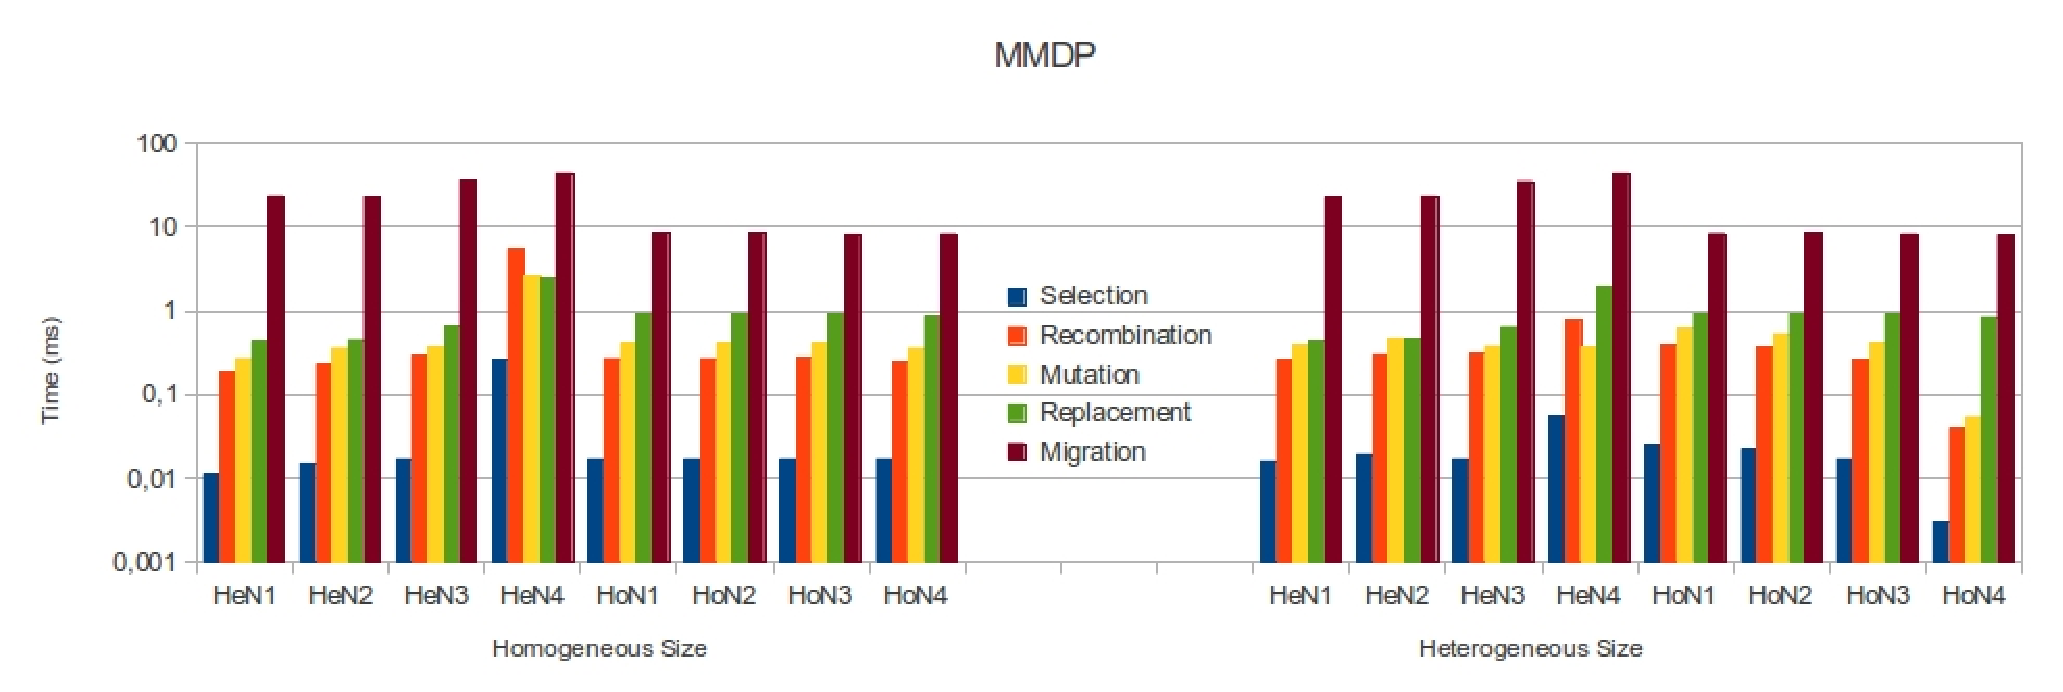
\epsfig{file=figure11.eps, width = 17cm}
\caption{Average running time in each stage of the algorithm for the MMDP problem.}
\label{fig:MMDPbars}
\end{figure*}

\begin{figure*}
\centering
\epsfig{file=figure12.eps, width = 17cm}
\caption{Average running time in each stage of the algorithm for the ONEMAX problem.}
\label{fig:ONEMAXbars}
\end{figure*}

\begin{table*}
\centering
\caption{Times of the stages of the algorithm for the MMDP problem (in ms).}
\begin{tabular}{|c|c|c|c|c|c|} \hline
\multicolumn{6}{|c|}{Homogeneous Size} \\ \hline
Node	& Selection		& Recombination		& Mutation		& Replacement		& Migration	        \\ \hline
HeN1	& 0,011 $\pm$ 0,023	& 0,181	$\pm$ 0,149	& 0,269	$\pm$ 0,064	& 0,429	$\pm$ 4,873	& 23,097 $\pm$ 	31,917 \\ \hline
HeN2	& 0,015	$\pm$ 0,009	& 0,231	$\pm$ 0,116	& 0,357	$\pm$ 0,043	& 0,449	$\pm$ 5,214	& 22,928 $\pm$ 	35,187 \\ \hline
HeN3	& 0,017	$\pm$ 0,016	& 0,291	$\pm$ 0,132	& 0,372	$\pm$ 0,117	& 0,655	$\pm$ 6,533	& 36,139 $\pm$ 	38,434 \\ \hline
HeN4	& 0,257	$\pm$ 0,371	& 5,381	$\pm$ 14,941	& 2,556	$\pm$ 1,611	& 2,400	$\pm$ 5,588	& 43,490 $\pm$ 	9,475 \\ \hline \hline
HoN1	& 0,017	$\pm$ 0,016	& 0,268	$\pm$ 0,555	& 0,405	$\pm$ 0,051	& 0,913	$\pm$ 1,350	& 8,428	$\pm$ 5,276 \\ \hline
HoN2	& 0,017	$\pm$ 0,029	& 0,267	$\pm$ 0,409	& 0,405	$\pm$ 0,037	& 0,911	$\pm$ 1,419	& 8,441	$\pm$ 4,869 \\ \hline
HoN3	& 0,017	$\pm$ 0,021	& 0,272	$\pm$ 0,589	& 0,404	$\pm$ 0,249	& 0,914	$\pm$ 1,420	& 8,177	$\pm$ 4,072 \\ \hline
HoN4	& 0,017	$\pm$ 0,010	& 0,247	$\pm$ 0,479	& 0,356	$\pm$ 0,042	& 0,857	$\pm$ 1,636	& 8,284	$\pm$ 4,770 \\ \hline
\multicolumn{6}{|c|}{Heterogeneous Size} \\ \hline									
Node	& Selection		& Recombination		& Mutation		& Replacement		& Migration	\\ \hline
HeN1	& 0,016	$\pm$ 0,012	& 0,259	$\pm$ 0,402	& 0,384	$\pm$ 0,086	& 0,435	$\pm$ 4,760	& 22,389 $\pm$ 	31,184 \\ \hline
HeN2	& 0,019	$\pm$ 0,015	& 0,297	$\pm$ 0,408	& 0,467	$\pm$ 0,256	& 0,464	$\pm$ 4,956	& 23,044 $\pm$ 	32,704 \\ \hline
HeN3	& 0,017	$\pm$ 0,016	& 0,303	$\pm$ 0,522	& 0,376	$\pm$ 0,118	& 0,634	$\pm$ 6,156	& 34,804 $\pm$ 	35,557 \\ \hline
HeN4	& 0,055	$\pm$ 0,161	& 0,769	$\pm$ 4,056	& 0,361	$\pm$ 0,653	& 1,957	$\pm$ 8,160	& 43,300 $\pm$ 	26,672 \\ \hline \hline
HoN1	& 0,025	$\pm$ 0,017	& 0,389	$\pm$ 0,676	& 0,603	$\pm$ 0,060	& 0,929	$\pm$ 1,300	& 8,396	$\pm$ 4,147 \\ \hline
HoN2	& 0,022	$\pm$ 0,017	& 0,362	$\pm$ 0,523	& 0,530	$\pm$ 0,228	& 0,921	$\pm$ 1,265	& 8,498	$\pm$ 4,694 \\ \hline
HoN3	& 0,017	$\pm$ 0,011	& 0,259	$\pm$ 0,558	& 0,403	$\pm$ 0,050	& 0,916	$\pm$ 1,409	& 8,250	$\pm$ 4,516 \\ \hline
HoN4	& 0,003	$\pm$ 0,005	& 0,039	$\pm$ 0,333	& 0,054	$\pm$ 0,029	& 0,836	$\pm$ 1,513	& 8,089	$\pm$ 4,602 \\ \hline
\end{tabular}
\label{tab:mmdptimes}
\end{table*}

\begin{table*}
\centering
\caption{Times of the stages of the algorithm for the OneMax problem (in ms).}
\begin{tabular}{|c|c|c|c|c|c|} \hline
\multicolumn{6}{|c|}{Homogeneous Size} \\ \hline
Node	& Selection		& Recombination		& Mutation		& Replacement		& Migration	        \\ \hline
HeN1	& 0,014	$\pm$ 0,016	& 4,063	$\pm$  3,290		& 7,826		$\pm$  	0,513	& 5,300 $\pm$ 62,474 &	328,262	$\pm$ 387,402 \\ \hline
HeN2	& 0,015	$\pm$ 0,019	& 4,221	$\pm$ 3,251			& 	8,325	$\pm$  	1,348	& 6,390	$\pm$ 71,926 &	398,119	$\pm$ 428,012 \\ \hline
HeN3	& 0,020	$\pm$ 0,022	& 8,896	$\pm$ 3,561			& 12,289	$\pm$  	0,393	& 6,505	$\pm$ 77,069 &	410,141	$\pm$ 480,055 \\ \hline
HeN4	& 0,362	$\pm$ 0,920	& 341,888$\pm$ 381,390		& 97,075	$\pm$  	119,923	& 3,638	$\pm$ 14,627 &	112,680	$\pm$ 43,776 \\ \hline \hline
HoN1	& 0,021	$\pm$ 0,013	& 6,181	$\pm$ 2,386			& 11,545	$\pm$  	0,468	& 1,506	$\pm$ 3,642	& 28,355	$\pm$ 8,606 \\ \hline
HoN2	& 0,021	$\pm$ 0,013	& 6,685	$\pm$ 1,927			& 11,779	$\pm$  	1,242	& 1,364	$\pm$ 2,437	& 18,034	$\pm$ 7,422 \\ \hline
HoN3	& 0,022	$\pm$ 0,016	& 6,154	$\pm$ 2,238			& 11,585	$\pm$  	0,506	& 1,363	$\pm$ 2,437	& 18,948	$\pm$ 6,072 \\ \hline
HoN4	& 0,021	$\pm$ 0,007	& 6,124	$\pm$ 2,346			& 11,560	$\pm$  	0,519	& 1,314	$\pm$ 2,308	& 17,920	$\pm$ 4,816 \\ \hline
\multicolumn{6}{|c|}{Heterogeneous Size} \\ \hline									
Node	& Selection		& Recombination		& Mutation		& Replacement		& Migration	\\ \hline
HeN1	& 0,017	$\pm$ 0,002	& 5,955	$\pm$ 3,569	    	& 11,761	$\pm$ 0,500		& 1,000	$\pm$ 11,748 & 50,470 $\pm$ 81,518 \\ \hline
HeN2	& 0,015	$\pm$ 0,002	& 5,448	$\pm$ 3,102			& 10,879	$\pm$ 1,545		& 0,972	$\pm$ 11,253 & 48,942 $\pm$ 77,468 \\ \hline
HeN3	& 0,016	$\pm$ 0,003	& 8,733	$\pm$ 2,180			& 11,672	$\pm$ 0,870		& 1,113	$\pm$ 7,352	& 59,133 $\pm$ 	8,825 \\ \hline
HeN4	& 0,040	$\pm$ 0,035	& 17,943 $\pm$ 23,543		& 10,751	$\pm$ 1,683		& 2,144	$\pm$ 9,815	& 76,816 $\pm$ 15,500 \\ \hline \hline
HoN1	& 0,032	$\pm$ 0,014	& 9,587 $\pm$ 	5,671		& 17,506	$\pm$ 1,083		& 1,482	$\pm$ 2,245	&17,121  $\pm$ 	6,302 \\ \hline
HoN2	& 0,027	$\pm$ 0,015	& 8,826	$\pm$ 5,850			& 15,262	$\pm$ 1,091		& 1,422	$\pm$ 2,766	&17,831	 $\pm$ 14,158 \\ \hline
HoN3	& 0,021	$\pm$ 0,013	& 6,108	$\pm$ 3,461			& 11,655	$\pm$ 0,534		& 1,365	$\pm$ 2,294  &17,440  $\pm$ 	6,578 \\ \hline
HoN4	& 0,004	$\pm$ 0,002	& 0,807	$\pm$ 0,749			& 1,653		$\pm$ 0,051		& 0,922	$\pm$ 2,672	&17,411	 $\pm$ 12,177 \\ \hline
\end{tabular}
\label{tab:onemaxtimes}
\end{table*}

\section{Conclusions}
% no cuentes otra vez lo de los computing trends, hombre. Empieza
% diciendo "in this paper we have introduced this o studied that" - JJ FERGU: Cambiada la introducción
%New computing trends, such as Cloud Computing or Service Oriented
%Architecture are providing a massively amount of heterogeneous
%computational devices. 
In this paper we have performed a study about adapting the
population size of an Evolutionary Algorithm to the computational
power of different nodes in an heterogeneous cluster. To obtain a fair parameter configuration,
this parameter has been obtained proportionally to the attained
average generations of each node in executions with the same number of
individuals. Results show that adapting the population size to the computational power decreases
the execution time significantly in heterogeneous clusters, while
changing this parameter in homogeneous clusters does not always
performs better. Moreover, changing this parameter affects to stages
of the algorithm that are independent of the population size, such as
the migration. These results are a promising start for adapting EAs to the
performance of each execution node. 
% Falta una discusión sobre si las mejoras se deben exclusivamente al
% número de evaluaciones o hay algún otro factor ¿menos overhead?
% ¿nodos más rápidos? - JJ FERGU: no, de hecho el número de evaluaciones no siempre disminuye, lo digo arriba.

In the future it would be interesting to check the scalability of this
approach, using more computational nodes and larger problem
instances. In addition, other parameters such as migration rate or
crossover probability could be adapted to the execution
nodes. Different benchmarks will be also used to lead to automatic
parameter adaptation in runtime, with different nodes entering or
exiting in the topology, or adapting to the current load of the
system. 



\begin{acknowledgements}
This work has been supported in part by FPU research grant AP2009-2942 and projects EvOrq (TIC-3903), SINECA (0100DGT21285, Spanish Direccion General de Trafico) and TIN2011-28627-C04-02.
\end{acknowledgements}

%\bibliographystyle{plain} %No spbasic
%\bibliography{heterogeneous} 

\begin{thebibliography}{10}

\bibitem{EVALUATIONPARALLEL}
E.~Alba and G.~Luque.
\newblock Evaluation of parallel metaheuristics.
\newblock In Springer, editor, {\em Parallel Problem Solving from Nature
  (PPSN)}, volume 4193 of {\em LNCS}, pages 9--14, 2006.

\bibitem{HETEROGENEOUSHARD}
Enrique Alba, Antonio~J. Nebro, and Jos\'e~M. Troya.
\newblock Heterogeneous computing and parallel genetic algorithms.
\newblock {\em Journal of Parallel and Distributed Computing}, 62(9):1362 --
  1385, 2002.

\bibitem{OPENSCIENCEGRID}
Mine Altunay, Paul Avery, Kent Blackburn, Brian Bockelman, Michael Ernst, Dan
  Fraser, Robert Quick, Robert Gardner, Sebastien Goasguen, Tanya Levshina,
  Miron Livny, John McGee, Doug Olson, Ruth Pordes, Maxim Potekhin, Abhishek
  Rana, Alain Roy, Chander Sehgal, Igor Sfiligoi, Frank Wuerthwein, and {Open
  Sci Grid Executive Board}.
\newblock {A Science Driven Production Cyberinfrastructure-the Open Science
  Grid}.
\newblock {\em {Journal of GRID Computing}}, {9}({2, Sp. Iss. SI}):{201--218},
  {JUN} 2011.

\bibitem{MULTIKULTI}
Lourdes Araujo and Juan Juli{\'a}n~Merelo Guerv{\'o}s.
\newblock Diversity through multiculturality: Assessing migrant choice policies
  in an island model.
\newblock {\em IEEE Trans. Evolutionary Computation}, 15(4):456--469, 2011.

\bibitem{SELFSTAR}
O.~Babaoglu, M.~Jelasity, A.~Montresor, C.~Fetzer, S.~Leonardi, and A.~van
  Moorsel.
\newblock {The self-star vision}.
\newblock {\em Self-star Properties in Complex Information Systems}, pages
  1--20, 2005.

\bibitem{CLOUD}
Rajkumar Buyya, Chee~Shin Yeo, Srikumar Venugopal, James Broberg, and Ivona
  Brandic.
\newblock Cloud computing and emerging it platforms: Vision, hype, and reality
  for delivering computing as the 5th utility.
\newblock {\em Future Gener. Comput. Syst.}, 25:599--616, June 2009.

\bibitem{TUTORIAL}
Joaqu\'{\i}n Derrac, Salvador Garc\'{\i}a, Daniel Molina, and Francisco
  Herrera.
\newblock A practical tutorial on the use of nonparametric statistical tests as
  a methodology for comparing evolutionary and swarm intelligence algorithms.
\newblock {\em Swarm and Evolutionary Computation}, 1(1):3--18, 2011.

\bibitem{HYDROCM}
Juli\'an Dom\'inguez and Enrique Alba.
\newblock {HydroCM}: A hybrid parallel search model for heterogeneous
  platforms.
\newblock In El-Ghazali Talbi, editor, {\em Hybrid Metaheuristics}, volume 434
  of {\em Studies in Computational Intelligence}, pages 219--235. Springer
  Berlin Heidelberg, 2013.

\bibitem{CELLULAR}
Bernab{\'e} Dorronsoro and Pascal Bouvry.
\newblock Cellular genetic algorithms without additional parameters.
\newblock {\em The Journal of Supercomputing}, 63:816--835, 2013.

\bibitem{PARAMETERTUNING}
A.~E. Eiben and Selmar~K. Smit.
\newblock Parameter tuning for configuring and analyzing evolutionary
  algorithms.
\newblock {\em Swarm and Evolutionary Computation}, 1(1):19--31, 2011.

\bibitem{GLOBUS}
I~Foster.
\newblock {Globus Toolkit version 4: Software for service-oriented systems}.
\newblock In {Jin, H and Reed, D and Jiang, W}, editor, {\em {Network and
  Parallel Computing Proceedings}}, volume {3779} of {\em {Lecture Notes in
  Computer Science}}, pages {2--13}, 2005.

\bibitem{GENERICITY05}
C.~Gagn{\'e} and M.~Parizeau.
\newblock Genericity in evolutionary computation software tools: Principles and
  case-study.
\newblock {\em International Journal on Artificial Intelligence Tools},
  15(2):173, 2006.

\bibitem{PARALLELIMPLEMENTATION}
J.F. Garamendi and J.L. Bosque.
\newblock Parallel implementation of evolutionary strategies on heterogeneous
  clusters with load balancing.
\newblock In {\em Parallel and Distributed Processing Symposium, 2006. IPDPS
  2006. 20th International}, page 8 pp., april 2006.

\bibitem{SOASOCO}
P.~Garc{\'i}a-S{\'a}nchez, J.~Gonz{\'a}lez, P.A. Castillo, M.G. Arenas, and
  J.J. Merelo-Guerv{\'o}s.
\newblock Service oriented evolutionary algorithms.
\newblock {\em Soft Computing}, pages 1--17, 2013.
\newblock 10.1007/s00500-013-0999-5.

\bibitem{goldberg92massive}
David~E. Goldberg, Kalyanmoy Deb, and Jeffrey Horn.
\newblock Massive multimodality, deception, and genetic algorithms.
\newblock In {R. M\"{a}nner} and B.~Manderick, editors, {\em Parallel Problem
  Solving from Nature, 2}, pages 37--48, Amsterdam, 1992. Elsevier Science
  Publishers, B. V.

\bibitem{HETEROGENEOUSPARAMETERS}
Yiyuan Gong and Alex Fukunaga.
\newblock Distributed island-model genetic algorithms using heterogeneous
  parameter settings.
\newblock In {\em Proceedings of the IEEE Congress on Evolutionary Computation,
  CEC 2011, New Orleans, LA, USA, 5-8 June, 2011}, pages 820--827. IEEE, 2011.

\bibitem{HETEROGENEOUSTOPOLOGY}
Yiyuan Gong, Morikazu Nakamura, and Shiro Tamaki.
\newblock Parallel genetic algorithms on line topology of heterogeneous
  computing resources.
\newblock In {\em Proceedings of the 2005 conference on Genetic and
  evolutionary computation}, GECCO '05, pages 1447--1454, New York, NY, USA,
  2005. ACM.

\bibitem{NUCLEAR}
Antonio G{\'o}mez-Iglesias, Miguel A. Vega-Rodr{\'i}guez, Francisco Castej{\'o}n-Maga{\~n}a,
  Miguel C{\'a}rdenas-Montes, and Enrique Morales-Ramos.
\newblock Evolutionary computation and grid computing to optimise nuclear
  fusion devices.
\newblock {\em Cluster Computing}, 12:439--448, 2009.

\bibitem{SURVEYMOFS}
José Parejo, Antonio Ruiz-Cort{\'e}s, Sebastián Lozano, and Pablo Fernandez.
\newblock Metaheuristic optimization frameworks: a survey and benchmarking.
\newblock {\em Soft Computing - A Fusion of Foundations, Methodologies and
  Applications}, 16:527--561, 2012.
\newblock 10.1007/s00500-011-0754-8.

\bibitem{PLATO}
Andres~J. Ramirez, David~B. Knoester, Betty H.~C. Cheng, and Philip~K.
  McKinley.
\newblock Plato: a genetic algorithm approach to run-time reconfiguration in
  autonomic computing systems.
\newblock {\em Cluster Computing}, 14(3):229--244, 2011.

\bibitem{HETEROGENEOUSMIGRATION}
Carolina Salto and Enrique Alba.
\newblock Designing heterogeneous distributed gas by efficiently self-adapting
  the migration period.
\newblock {\em Applied Intelligence}, 36:800--808, 2012.

\bibitem{ONEMAX}
J.D. Schaffer and L.J. Eshelman.
\newblock {On Crossover as an Evolutionary Viable Strategy}.
\newblock In R.K. Belew and L.B. Booker, editors, {\em {Proceedings of the 4th
  International Conference on Genetic Algorithms}}, pages 61--68. Morgan
  Kaufmann, 1991.

\end{thebibliography}



\end{document}
% end of file template.tex

